%%%%%%%%%%%%%%%%%%%%%%%%%%%%%%%%%%%%%%%%%%%%%%%%%%%%%%%%%%%%%%%%%%%%%%%%%%%%%%%
%%  claude-giga-lens-linus --- TECHNICAL REPORT, SECTION FILE A.
%%
%%  Front matter (title/abstract) + Introduction + Methods I/II/III.
%%  To be \input{} into papers/main.tex AFTER \begin{document}; assumes the
%%  companion report's preamble (tech-report.sty, natbib, and the macro set of
%%  ../claude-giga-lens/papers/main.tex).  A \providecommand compatibility
%%  block below makes this file safe even if some macros are absent.
%%
%%  Every number in this file is traced to an artifact path per the campaign
%%  spine (research/synthesis_tables.md); its seven DISCREPANCY FLAGS are
%%  binding and the ARTIFACT value is quoted wherever ledger prose disagrees
%%  (e.g. the MCLMC bias screen is 20.1-sigma, not the ledger's "30-sigma").
%%
%%  Section labels in this file are unique with the "-a" suffix:
%%    sec:intro-a, sec:substrate-a, sec:port-a, sec:protocol-a
%%    tab:gates-a, tab:pins-a
%%
%%  BIB KEYS: reuses the companion report's references.bib keys
%%  (gu2022gigalens, huang2026gigalens2, huang2025foundry1,
%%   etherington2024codecomparison, blackjax2024, robnik2023mclmc,
%%   bradbury2018jax, dillon2017tfp).  FOUR NEW KEYS are cited here and must
%%  be added to references.bib -- suggested entries:
%%
%%  @techreport{cgl2026companion,
%%    author = {Benson, Greg and Huang, Xiaosheng},
%%    title  = {Correlated-Noise Likelihoods and Next-Generation Inference
%%              for Strong Gravitational Lens Modeling},
%%    institution = {University of San Francisco},
%%    year   = {2026}, month = jul,
%%    note   = {Technical report, campaign claude-giga-lens; commit 4003aac}}
%%  @article{delmoral2006smc,
%%    author = {Del Moral, Pierre and Doucet, Arnaud and Jasra, Ajay},
%%    title  = {Sequential {M}onte {C}arlo samplers},
%%    journal = {Journal of the Royal Statistical Society: Series B},
%%    volume = {68}, number = {3}, pages = {411--436}, year = {2006}}
%%  @misc{robnik2024mams,
%%    author = {Robnik, Jakob and Seljak, Uro{\v s}},
%%    title  = {Metropolis-Adjusted Microcanonical Sampler},
%%    year   = {2024},
%%    note   = {arXiv preprint; verify final id/venue before publication}}
%%  @misc{talts2018sbc,
%%    author = {Talts, Sean and Betancourt, Michael and Simpson, Daniel and
%%              Vehtari, Aki and Gelman, Andrew},
%%    title  = {Validating {B}ayesian Inference Algorithms with
%%              Simulation-Based Calibration},
%%    year   = {2018}, note = {arXiv:1804.06788}}
%%%%%%%%%%%%%%%%%%%%%%%%%%%%%%%%%%%%%%%%%%%%%%%%%%%%%%%%%%%%%%%%%%%%%%%%%%%%%%%

% --- Compatibility block: no-ops if the shared preamble already defines them.
\providecommand{\thetaE}{\ensuremath{\theta_{\mathrm{E}}}}
\providecommand{\gammaEPL}{\ensuremath{\gamma}}
\providecommand{\Rhat}{\ensuremath{\hat{R}}}
\providecommand{\ESS}{\textrm{ESS}}
\providecommand{\eop}{\ensuremath{e_{\mathrm{op}}}}
\providecommand{\gigalens}{\textsc{GIGA-Lens}}
\providecommand{\gigalenstwo}{\textsc{GIGA-Lens\,2.0}}
\providecommand{\foundry}{DESI--165.4754$-$06.0423}
\providecommand{\blackjax}{\textsc{BlackJAX}}
\providecommand{\art}[1]{\footnote{Source artifact: \texttt{#1}.}}
\providecommand{\dfile}[1]{\texttt{#1}}
\providecommand{\subtitle}[1]{\begin{center}\large\itshape #1\end{center}}
% --- Macros local to this report (guarded).
\providecommand{\sboot}{\ensuremath{\sigma_{\mathrm{boot}}}}
\providecommand{\sseed}{\ensuremath{\sigma_{\mathrm{seed}}}}
\providecommand{\logZ}{\ensuremath{\log Z}}
\providecommand{\dlogZ}{\ensuremath{\Delta\log Z}}
\providecommand{\sceneapi}{scene API}
\providecommand{\vendorpin}{\texttt{80916d2}}

\title{Bridging a Correlated-Noise Likelihood and Evidence-Based Inference
       onto the Next-Generation \gigalens\ Scene API:\\
       a Certification, Benchmark, and Mechanism Campaign\thanks{All work
       reported here --- code, experiments, analysis, and text --- was
       performed by Claude Code (Anthropic), guided by Greg Benson. This
       document is a technical report. Results obtained on the scene-API
       substrate are labeled \emph{proposed (UNCERTIFIED --- external)}
       throughout: we are the producer; the grader is the upstream
       \gigalens\ development team (\S\ref{sec:protocol-a}). Co-authorship
       on any publication whose results run through that substrate is
       offered to the team; their sign-off gates all such material.}}
\author{Greg Benson\thanks{Department of Computer Science, University of
        San Francisco, CA 94117, USA; \texttt{greg.benson@gmail.com}.}}
\date{July 2026\\[3pt]{\small\texttt{commit:~3bc5f9d}}}

\maketitle
\subtitle{Technical report: campaign \texttt{claude-giga-lens-linus},
experimental program complete 2026-07-21 (53.51 of 100 A100\,h);
companion to \citet{cgl2026companion}}

\begin{abstract}
Our companion campaign \citep{cgl2026companion} closed with a two-sided
verdict on the real {\it HST}/WFC3-IR lens \foundry: a drizzle-anchored
correlated-noise likelihood is \emph{necessary but not sufficient} --- it
flips the binned-product bimodality (a $\sim$191-nat per-basin evidence
swing, exposing the steep basin as a noise-covariance artifact) yet
over-corrects the slope to $\gammaEPL=1.103\pm0.008$, $\sim$$17\sigma$ below
the $1.433$ native-diagonal anchor --- and with the finding that real
ill-conditioned and bimodal lens posteriors need a two-stage preconditioned
recipe plus per-basin SMC evidence. Meanwhile the \gigalens\ team's
next-generation rewrite (``the upstream development branches'') rebuilt the
forward model around a unified multi-plane, multi-band \emph{\sceneapi} whose
validation suite was, at the commit we vendored, not yet run, and which
contains neither a correlated-noise likelihood nor an evidence layer. This
report bridges the two lineages under a pre-registered, budget-fenced,
proposer$\ne$grader protocol (53.51 of a 100 A100\,h cap). The outcome is
deliberately two-sided. \emph{Delivered:} (i) the first external
certification of the \sceneapi\ forward model for the EPL+shear +
S\'ersic/shapelet configuration class --- machine-precision cross-stack
parity (forward image $5.7\times10^{-15}$; gradients $1.5\times10^{-11}$)
on both machines, with three documented convention reconciliations,
including a real $\sim$$2\times10^{-3}$ S\'ersic-$b_n$ approximant
difference, and an $\mathrm{fp}128$-referenced restatement of the Occam
log-determinant gate after the original cross-algorithm reference proved
noisier than the quantity it gated; (ii) a ported
\texttt{CorrelatedImageData} likelihood term, exact in its analytic limits,
that \emph{reproduces the money number cross-stack}: $\gammaEPL=1.1005$
(offset $0.0027$) with $\logZ$ agreement across stacks and machines to
$0.11$ nats in the low basin and $0.37$ nats in the steep ---
$\gammaEPL=1.103$ now stands on two independent
implementations; (iii) a sampler decision matrix from the first
microcanonical-SMC benchmark on lens posteriors: prior-seeded MAMS-SMC is
the only vehicle in the campaign that produced evidence at all (analytic
targets, a double-source-plane ridge at $\lambda{=}1$, both basins of a
74-dim bimodal target with retention $1.000$, and the correlated real-data
refit), and where it fails it fails \emph{by cost, never by health} ---
every non-completion is a wall-cap on a healthy sampler; on the 33-dim
multi-plane real-data cell (MUSE cutouts provided by the team, used with
permission) \emph{neither} cold-start SMC nor warm MAMS converges at
matched budget, while the classic single-stage MAP$\to$SVI$\to$HMC recipe
produced no accepted posterior anywhere in the campaign, reproducing the
known single-stage pathology on the new substrate. Unadjusted-MCLMC
mutations are demoted for evidence work: a $20.1\sigma$ bias screen and a
measured $\times56$ minor-mode evidence inflation that SMC resampling does
not launder at point estimate. Two cross-cutting negatives bind future evidence claims:
bootstrap $\logZ$ errors understate true errors (measured $+3.06\pm0.35$
nats where the truth is $\approx$0), and a frozen MCMC-derived reference
was itself indicted by an $11\sigma$ gate failure whose decomposition shows
both basins with \emph{more} evidence and $\gammaEPL$-disjoint support ---
frozen references need coverage certificates. \emph{Bounded, not decided:}
the anchor arbitration (does $1.433$ reproduce end-to-end on the new
substrate?) closed PARTIAL-BY-VEHICLE-EXHAUSTION with no quotable
$\gammaEPL$. \emph{Rejected:} stationarity of the noise-model class behind
$\gammaEPL=1.103$ (calibrated $p=0.010$; cross-block kernel spread
$16.4\times$ the drizzle-registration envelope) --- the standing working
hypothesis for the over-correction, unconfirmed but unrefuted after the
injection-recovery test was confounded by scene-subtraction residue.
Every quantitative claim traces to a JSON artifact, a job id, and a gate
row in \texttt{CAMPAIGN.md}.
\end{abstract}

% Up-front digest for lens modelers (added in response to the GIGA-Lens
% team's review of the report): the five standard checks, placed ahead of
% the Introduction. Lives in its own section file.
%%%%%%%%%%%%%%%%%%%%%%%%%%%%%%%%%%%%%%%%%%%%%%%%%%%%%%%%%%%%%%%%%%%%%%%%%%%%%%%
%%  claude-giga-lens-linus --- SUMMARY FOR LENS MODELERS (up-front section).
%%
%%  \input directly after the abstract (before the Introduction), in response
%%  to the GIGA-Lens team's review: the five things a lens modeler checks
%%  first, collected in one place.  Structured exactly as the five requested
%%  items: (1) data/model/residual + critical curves & caustics; (2) reduced
%%  chi^2; (3) sampling method; (4) convergence metrics; (5) corner plot.
%%
%%  Every number is quoted from its on-disk artifact per the campaign spine
%%  (research/synthesis_tables.md; its seven DISCREPANCY FLAGS are binding).
%%  The whitened reduced chi^2 was not stored by any production artifact and
%%  was recomputed for this section at the identical posterior-median model
%%  point on the validated old stack, bit-matching the head-to-head artifact's
%%  gamma AND whitened logL before being quoted
%%  (data/summary_rchi2_whitened_corrlow.json).
%%
%%  ASSEMBLY NOTE: the figure environments for \ref{fig:critcurves}
%%  (critical curves / caustics) and \ref{fig:corner} (posterior corner) are
%%  produced by the figure lane; place them in or near this section.  All
%%  other \ref targets exist in sections A--C.
%%%%%%%%%%%%%%%%%%%%%%%%%%%%%%%%%%%%%%%%%%%%%%%%%%%%%%%%%%%%%%%%%%%%%%%%%%%%%%%

% Guarded local shorthands (harmless if already defined by the preamble).
\providecommand{\sboot}{\ensuremath{\sigma_{\mathrm{boot}}}}
\providecommand{\sseed}{\ensuremath{\sigma_{\mathrm{seed}}}}
\providecommand{\logZ}{\ensuremath{\log Z}}
\providecommand{\dlogZ}{\ensuremath{\Delta\log Z}}

%%%%%%%%%%%%%%%%%%%%%%%%%%%%%%%%%%%%%%%%%%%%%%%%%%%%%%%%%%%%%%%%%%%%%%%%%%%%%%%
\section{Summary for Lens Modelers}
\label{sec:modelers}
%%%%%%%%%%%%%%%%%%%%%%%%%%%%%%%%%%%%%%%%%%%%%%%%%%%%%%%%%%%%%%%%%%%%%%%%%%%%%%%

This section collects, up front, the five things a lens modeler checks
first. Every number is quoted from its on-disk artifact (the campaign spine,
\dfile{research/synthesis\_tables.md}, binds); results on the \sceneapi\
substrate carry the report's \emph{proposed (UNCERTIFIED --- external)}
label. The system throughout is the real {\it HST}/WFC3-IR lens \foundry;
the three competing mass models are the native-diagonal \textbf{anchor}
($\gammaEPL=1.433\pm0.034$), the correlated-likelihood binned-low
\textbf{money number} ($\gammaEPL=1.1032\pm0.0086$), and the same-product
\textbf{diagonal-low} solution ($\gammaEPL=1.293\pm0.012$), the first and
third inherited from the companion campaign \citep{cgl2026companion}.

\paragraph{(1) Data, model, residual --- and the caustic structure.}
Figure~\ref{fig:headtohead} is the key diagnostic: data, model, and
residual$/\sigma$ for all three posterior-median models rendered on the
\emph{same} \dfile{v3b} binned pixels. The one-look read: the correlated
optimum ($\gammaEPL=1.103$) leaves a strong coherent lens-center residual
that its own whitened metric prices as ``probably correlated noise,'' while
in real space the binned data prefer the $\gammaEPL\approx1.29$ diagonal
solution (\S\ref{sec:t043}) --- our diagnosis is that $1.103$ is a
whitened-metric optimum standing on a stationarity assumption the field
measurably violates (\S\ref{sec:t041}). Figure~\ref{fig:critcurves}
completes the geometric view with the lens-plane critical curves and
source-plane caustics of the same three models (money-model
$\thetaE=2.624\pm0.005$), making the mass-model disagreement visible as
caustic structure rather than only as a slope number.

\begin{figure}[htbp]
\centering
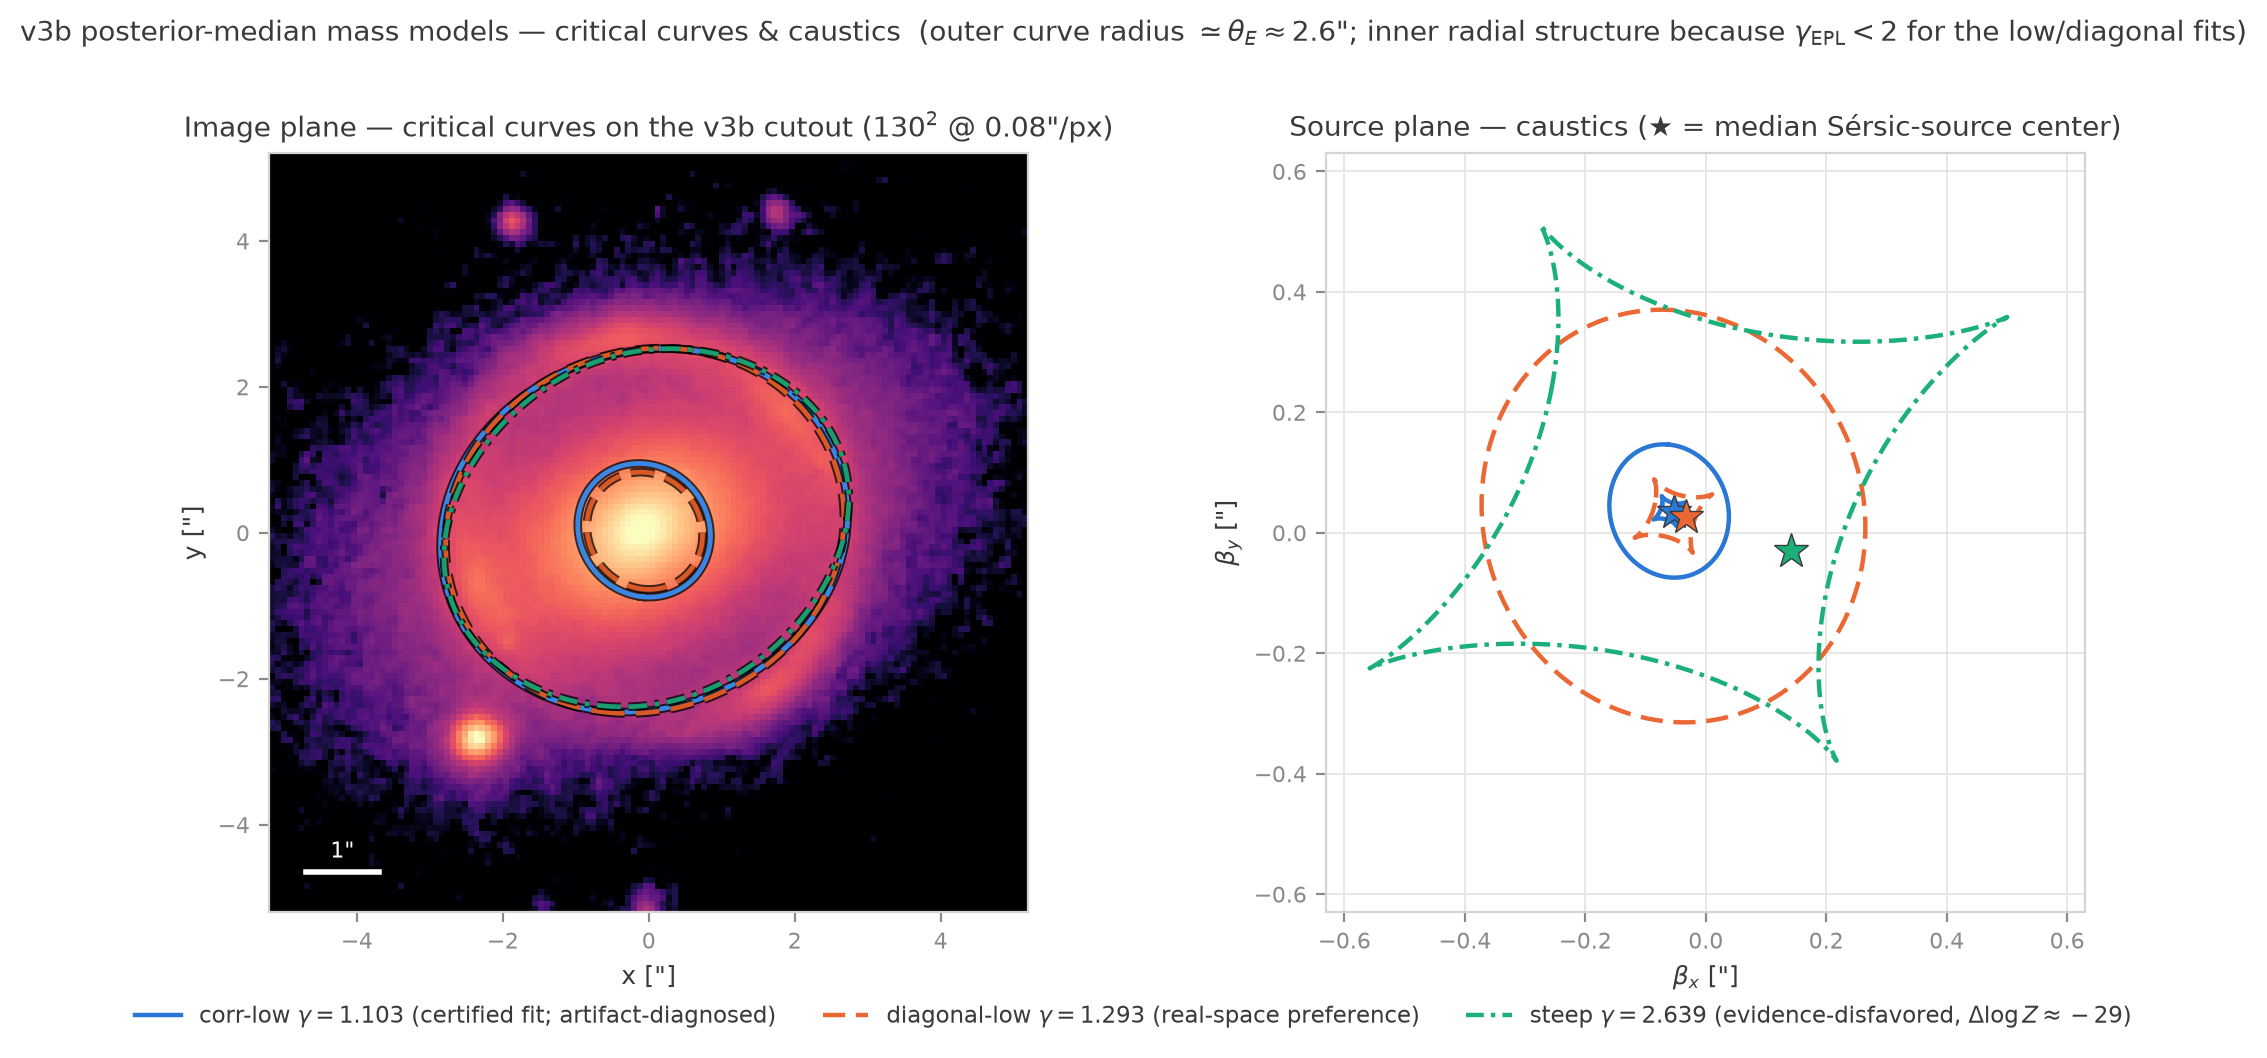
\includegraphics[width=0.98\textwidth]{../figs/rfig_critcurves.png}
\caption{Critical curves (lens plane, over the \dfile{v3b} binned cutout,
asinh stretch) and caustics (source plane; stars mark the median
S\'ersic-source centers) for the three posterior-median mass models,
following the critical-curve/caustic display conventions of the team's
\gigalens\ discovery paper \citep{gu2022gigalens}: corr-low
$\gammaEPL=1.103$ (the certified but artifact-diagnosed correlated fit),
diagonal-low $\gammaEPL=1.293$ (the real-space preference), and steep
$\gammaEPL=2.639$ (evidence-disfavored, $\dlogZ\approx-29$). Scale sanity:
the outer critical curve's median radius matches each model's \thetaE\ to
$<5\%$ (money model: $2.632''$ vs.\ $\thetaE=2.624''$), and the two
shallow ($\gammaEPL<2$) models show the expected inner radial critical
curve and caustic. Deflections from the vendored \sceneapi\ EPL(50)+shear
at the certified conventions; source artifact
\dfile{data/rfig\_modeler\_params.npz}.}
\label{fig:critcurves}
\end{figure}

\paragraph{(2) Reduced $\chi^2$ of the best-fit models.}
Table~\ref{tab:gof-modelers} gives both currencies. Under its own
production metric the money fit is formally excellent: whitened
$\chi^2/\mathrm{dof} = 8946.8/9273 = 0.965$ ($0.973$ after subtracting the
46 nonlinear + 28 marginalized-amplitude
parameters).\footnote{Source artifact:
\dfile{data/summary\_rchi2\_whitened\_corrlow.json} --- recomputed for this
section at the identical posterior-median model point on the validated
stack; it bit-matches the head-to-head artifact's $\gammaEPL$ and whitened
$\log L$ before being quoted.}
Two honest qualifiers frame the real-space column. First, \emph{this
field's own-model floor is $\approx1.6$, not $1.0$}: the injection-build
gate showed that even a ground-truth model of an injected scene scores
$\chi^2/\mathrm{px}=1.598$ full-keep versus $0.952$ on the sky subset ---
essentially all of the excess is bright-object scene-subtraction residue
(bright-object subset $2.71$, lens-center $r<1.2''$ subset
$5.46$)\art{data/t11\_injection\_build\_report.json;
data/t11b\_residue\_mask\_report.json;
data/t04\_realspace\_headtohead.json} --- so the diagonal-low value
$1.578$ \emph{is} the attainable field level, while $7.4$--$8.3$ for the
anchor and money models is genuine real-space misfit (the anchor row also
carries a cross-product resolution handicap: the same parameters render
$\chi^2/\mathrm{px}=1.251$ on their home native product). Second, the
whitened $0.965$ inherits the whitened metric's known caveat: its
stationary kernel class is \emph{rejected} by the field at calibrated
$p=0.010$ (\S\ref{sec:t041}), and the same metric prefers the money model
over diagonal-low by $+63$~nats in $\log L$ ($+501$ in log-posterior),
inverting the real-space ordering --- a reduced $\chi^2$ of $0.965$ here
certifies internal consistency, not noise-model correctness.

\begin{table}[htbp]
\centering
\caption{Goodness of fit for the three best-fit models on the same
\dfile{v3b} binned pixels: real-space $\chi^2/\mathrm{px}$
(diagonal-solved amplitudes; 16{,}653 keep px full field, 7{,}825 px arc
band $r\in[1.2,4.2]''$) and, for the production correlated fit, the
whitened reduced $\chi^2$ over the 9{,}273 whitened dof. Whitened
$\log L$ for all three models is in Table~\ref{tab:headtohead}. Sources:
\dfile{data/t04\_realspace\_headtohead.json},
\dfile{data/summary\_rchi2\_whitened\_corrlow.json},
\dfile{data/t11\_injection\_build\_report.json}.}
\label{tab:gof-modelers}
\small
\begin{tabular}{lccc}
\toprule
model ($\gammaEPL$) & $\chi^2/\mathrm{px}$ full & $\chi^2/\mathrm{px}$ arc
band & whitened $\chi^2/\mathrm{dof}$ \\
\midrule
diag-low $1.293$ (home reference) & $\mathbf{1.578}$ & $\mathbf{1.929}$ & --- \\
anchor $1.433$ (from \dfile{v2d}; home $1.251$) & $7.436$ & $3.622$ & --- \\
corr-low $1.103$ (money) & $8.321$ & $2.756$ & $\mathbf{0.965}$ \\
\midrule
\multicolumn{4}{@{}l@{}}{\footnotesize field's own-model floor (truth model
of injected scene): full-keep $1.598$; sky subset $0.952$ ---} \\
\multicolumn{4}{@{}l@{}}{\footnotesize the excess over $1.0$ is
bright-object scene-subtraction residue, faced by every fit on this
product.} \\
\bottomrule
\end{tabular}
\end{table}

\paragraph{(3) Sampling method.}
In HMC-vs-MCLMC vocabulary: every headline fit in this report was sampled
by \emph{adaptive tempered SMC} \citep{delmoral2006smc} ($\lambda:0\to1$,
per-stage adaptive step targeting a weighted ESS of $0.7N$, per-stage
bootstrap \logZ) whose mutation kernel is \emph{MAMS --- the
Metropolis-adjusted variant of MCLMC}
\citep{robnik2023mclmc,robnik2024mams}: microcanonical (MCLMC) dynamics
made exact by a Metropolis accept/reject step, tuned to the MAMS paper's
target acceptance of $0.90$. It is therefore neither plain HMC nor raw
(unadjusted) MCLMC. The distinction is load-bearing: unadjusted-MCLMC
mutations were demoted at the correctness gate ($20.1\sigma$ evidence bias
on the ill-conditioned analytic target; a measured $\times56$ minor-mode
evidence inflation on the 74-d bimodal target), and everywhere the classic
single-stage MAP$\to$SVI$\to$HMC recipe ran in this campaign it failed its
own acceptance rule (Table~\ref{tab:conv-modelers}; full decision matrix
Table~\ref{tab:decision}, \S\ref{sec:matrix:classic},
\S\ref{sec:matrix:b3}) --- consistent with the companion finding that
these real lens posteriors need the two-stage re-preconditioned recipe
\citep{cgl2026companion}.

\paragraph{(4) Convergence metrics.}
SMC has no $\Rhat$; the honest analogues are independent-seed repeats,
the per-stage weighted-ESS floor maintained by the adaptive
$\lambda$-schedule, unique-particle retention after resampling, MAMS
acceptance against its $0.90$ target, and --- strongest of all --- the
cross-stack, cross-machine reproduction. Table~\ref{tab:conv-modelers} is
the consolidated convergence ledger for every fit quoted in this report,
with $\Rhat$/ESS given where classic MCMC arms ran (both are rejections,
reported as such). For the two inherited diagonal fits (anchor $1.433$,
diag-low $1.293$) the per-fit $\Rhat$/ESS live in the companion report's
campaign ledger \citep{cgl2026companion} and are cited, not re-derived
here. Table~\ref{tab:conv-modelers} covers the fits \emph{quoted} in this
report; Appendix~\ref{app:convergence} extends it to the complete per-fit
ledger --- one row for every fit the campaign ever ran, including the
failed, rejected, collapsed, and budget-blocked arms.

\begin{table}[htbp]
\centering
\caption{Consolidated convergence ledger. wESS = final-stage weighted ESS;
``unique'' = unique particles after resampling; the adaptive
$\lambda$-schedule holds per-stage wESS at $0.7N$ by construction. Sources:
\dfile{data/t02\_t03\_gate\_eval.json} (+ per-seed run JSONs),
\dfile{data/results-perlmutter/l0g2\_v3b\_scene\_seed2.json},
\dfile{data/b1r\_decision\_matrix.json} +
\dfile{research/checkpoint\_b1r\_close.md},
\dfile{data/results-perlmutter/l0\_arbitration\_classic.json},
\dfile{data/b3\_run\_ref\_sys\{0..3\}\_l4-8.json},
\citet{cgl2026companion}.}
\label{tab:conv-modelers}
\scriptsize
\setlength{\tabcolsep}{3.5pt}
\renewcommand{\arraystretch}{1.3}
\begin{tabular}{@{}p{0.21\textwidth}p{0.135\textwidth}p{0.37\textwidth}p{0.21\textwidth}@{}}
\toprule
fit / arm & vehicle, $n$ & diagnostics & verdict \\
\midrule
\dfile{v3b} corr \textbf{low} ---
$\gammaEPL=1.1032\pm0.0086$ (\textbf{money}) &
tempered SMC + MAMS; 3 seeds $\times$ 128 &
$\lambda{=}1$ @28 stages every seed; wESS 118--128/128; unique 77--82/128;
seeds $\{1.1032, 1.0967, 1.1005\}$ $\Rightarrow$
$\sseed(\gammaEPL)=0.00325$, $\sseed(\logZ)=1.22$ nats &
\textbf{converged + seed-certified} (T0.2, \S\ref{sec:t02}); $n{=}3$
caveat: $\pm46\%$ on $\sseed$ itself \\
\dfile{v3b} corr steep ($\gammaEPL\approx2.64$) &
same; 3 seeds $\times$ 96 &
$\lambda{=}1$ @21--22 stages; wESS 36--96/96 (seed-2 final resample low);
unique 50--59/96; $\sseed(\gammaEPL)=0.00664$ &
converged; $\dlogZ(\mathrm{steep}-\mathrm{low})=-28.9/-32.3/-31.2$
seed-stable \\
same fit, \sceneapi\ port, Perlmutter A100 (L0-G2) &
same; 1 seed &
$\lambda{=}1$ @27/22 stages; wESS 123.5/128 (low), 47.6/96 (steep);
unique 81/128, 54/96 &
\textbf{PASS}: $\Delta\gammaEPL=0.0027$; \logZ\ agreement 0.11
(low)\,/\,0.37 (steep) nats \emph{across stacks and machines}
(\S\ref{sec:l0g2}) \\
carousel 33-d multi-plane REAL (B1r; hardest cell) &
same; 1 seed $\times$ 128 &
$\lambda=0.151$ @36 stages; unique 92--104/128 every stage; MAMS accept
0.871--0.934 (mean 0.899 vs 0.90 target); stage wESS pinned at $0.7N$ &
\textbf{no posterior}: sampler healthy, killed by wall-cap --- a cost
verdict, not a convergence failure (\S\ref{sec:matrix:b1r}) \\
\midrule
classic MAP$\to$SVI$\to$HMC, warm, \dfile{v2d} (arbitration arm) &
50 chains, 250 burn-in/750 draws; escalated 500/1500 &
$\Rhat_{\rm worst}=44.3$ (escalated $11.7$) vs rule $<1.05$;
$\ESS_{\min}=53.6$ ($63.0$ escalated); all chains railed
$\gammaEPL\approx1.987\,[1.983,1.991]$ at the prior edge &
\textbf{NO-VERDICT}: $\gammaEPL$ not quotable; reproduces the known T2
single-stage pathology on the \sceneapi\ (\S\ref{sec:matrix:classic}) \\
classic reference chains, hs2 scenes $\times4$ (B3) &
frozen 50-chain recipe &
$\Rhat_{\rm worst}=4.36$--$7.87$; $\ESS_{\min}=63.7$--$83.9$ vs rule
$\Rhat<1.05 \wedge \ESS\ge200$ &
all 4 \textbf{rejected} by the pre-registered acceptance rule
(\S\ref{sec:matrix:b3}) \\
\midrule
anchor $1.433$ (\dfile{v2d} diag) and diag-low $1.293$ (\dfile{v3b} diag) &
companion campaign (two-stage re-preconditioned recipe) &
provenance row: per-fit $\Rhat$/\ESS\ ledgered in the companion report &
converged there; cited, not re-derived \citep{cgl2026companion} \\
\bottomrule
\end{tabular}
\end{table}

\paragraph{(5) The posterior.}
Figure~\ref{fig:corner} shows the posterior corner for the production
correlated \dfile{v3b} fit with the three seed repeats overlaid. The
read-out: the Einstein radius is tight and stable
($\thetaE=2.6239\pm0.0049$, a $0.2\%$ constraint) while the two basins
remain cleanly separated in $\gammaEPL$ (low $1.103$ vs.\ steep $2.64$)
with a seed-stable evidence preference for the low basin of
$\approx29$--$32$ nats; the seed overlays coincide within
$\sseed(\gammaEPL)=0.00325$, which is what licenses quoting
$\sigma_{\rm tot}=0.0086$ on the money number
(\S\ref{sec:t02}).\footnote{Source artifacts: companion
\dfile{data/results/e2\_v3b\_low\_smc\_canary\_fix.json};
\dfile{data/t02\_t03\_gate\_eval.json}.}
The number this posterior constrains, and the standing caveat on
interpreting it, are the subject of the rest of this report:
$\gammaEPL=1.1032\pm0.0086$ is certified, cross-stack reproduced --- and
diagnosed as an artifact of a stationary noise-model class the field
rejects.

\begin{figure}[htbp]
\centering
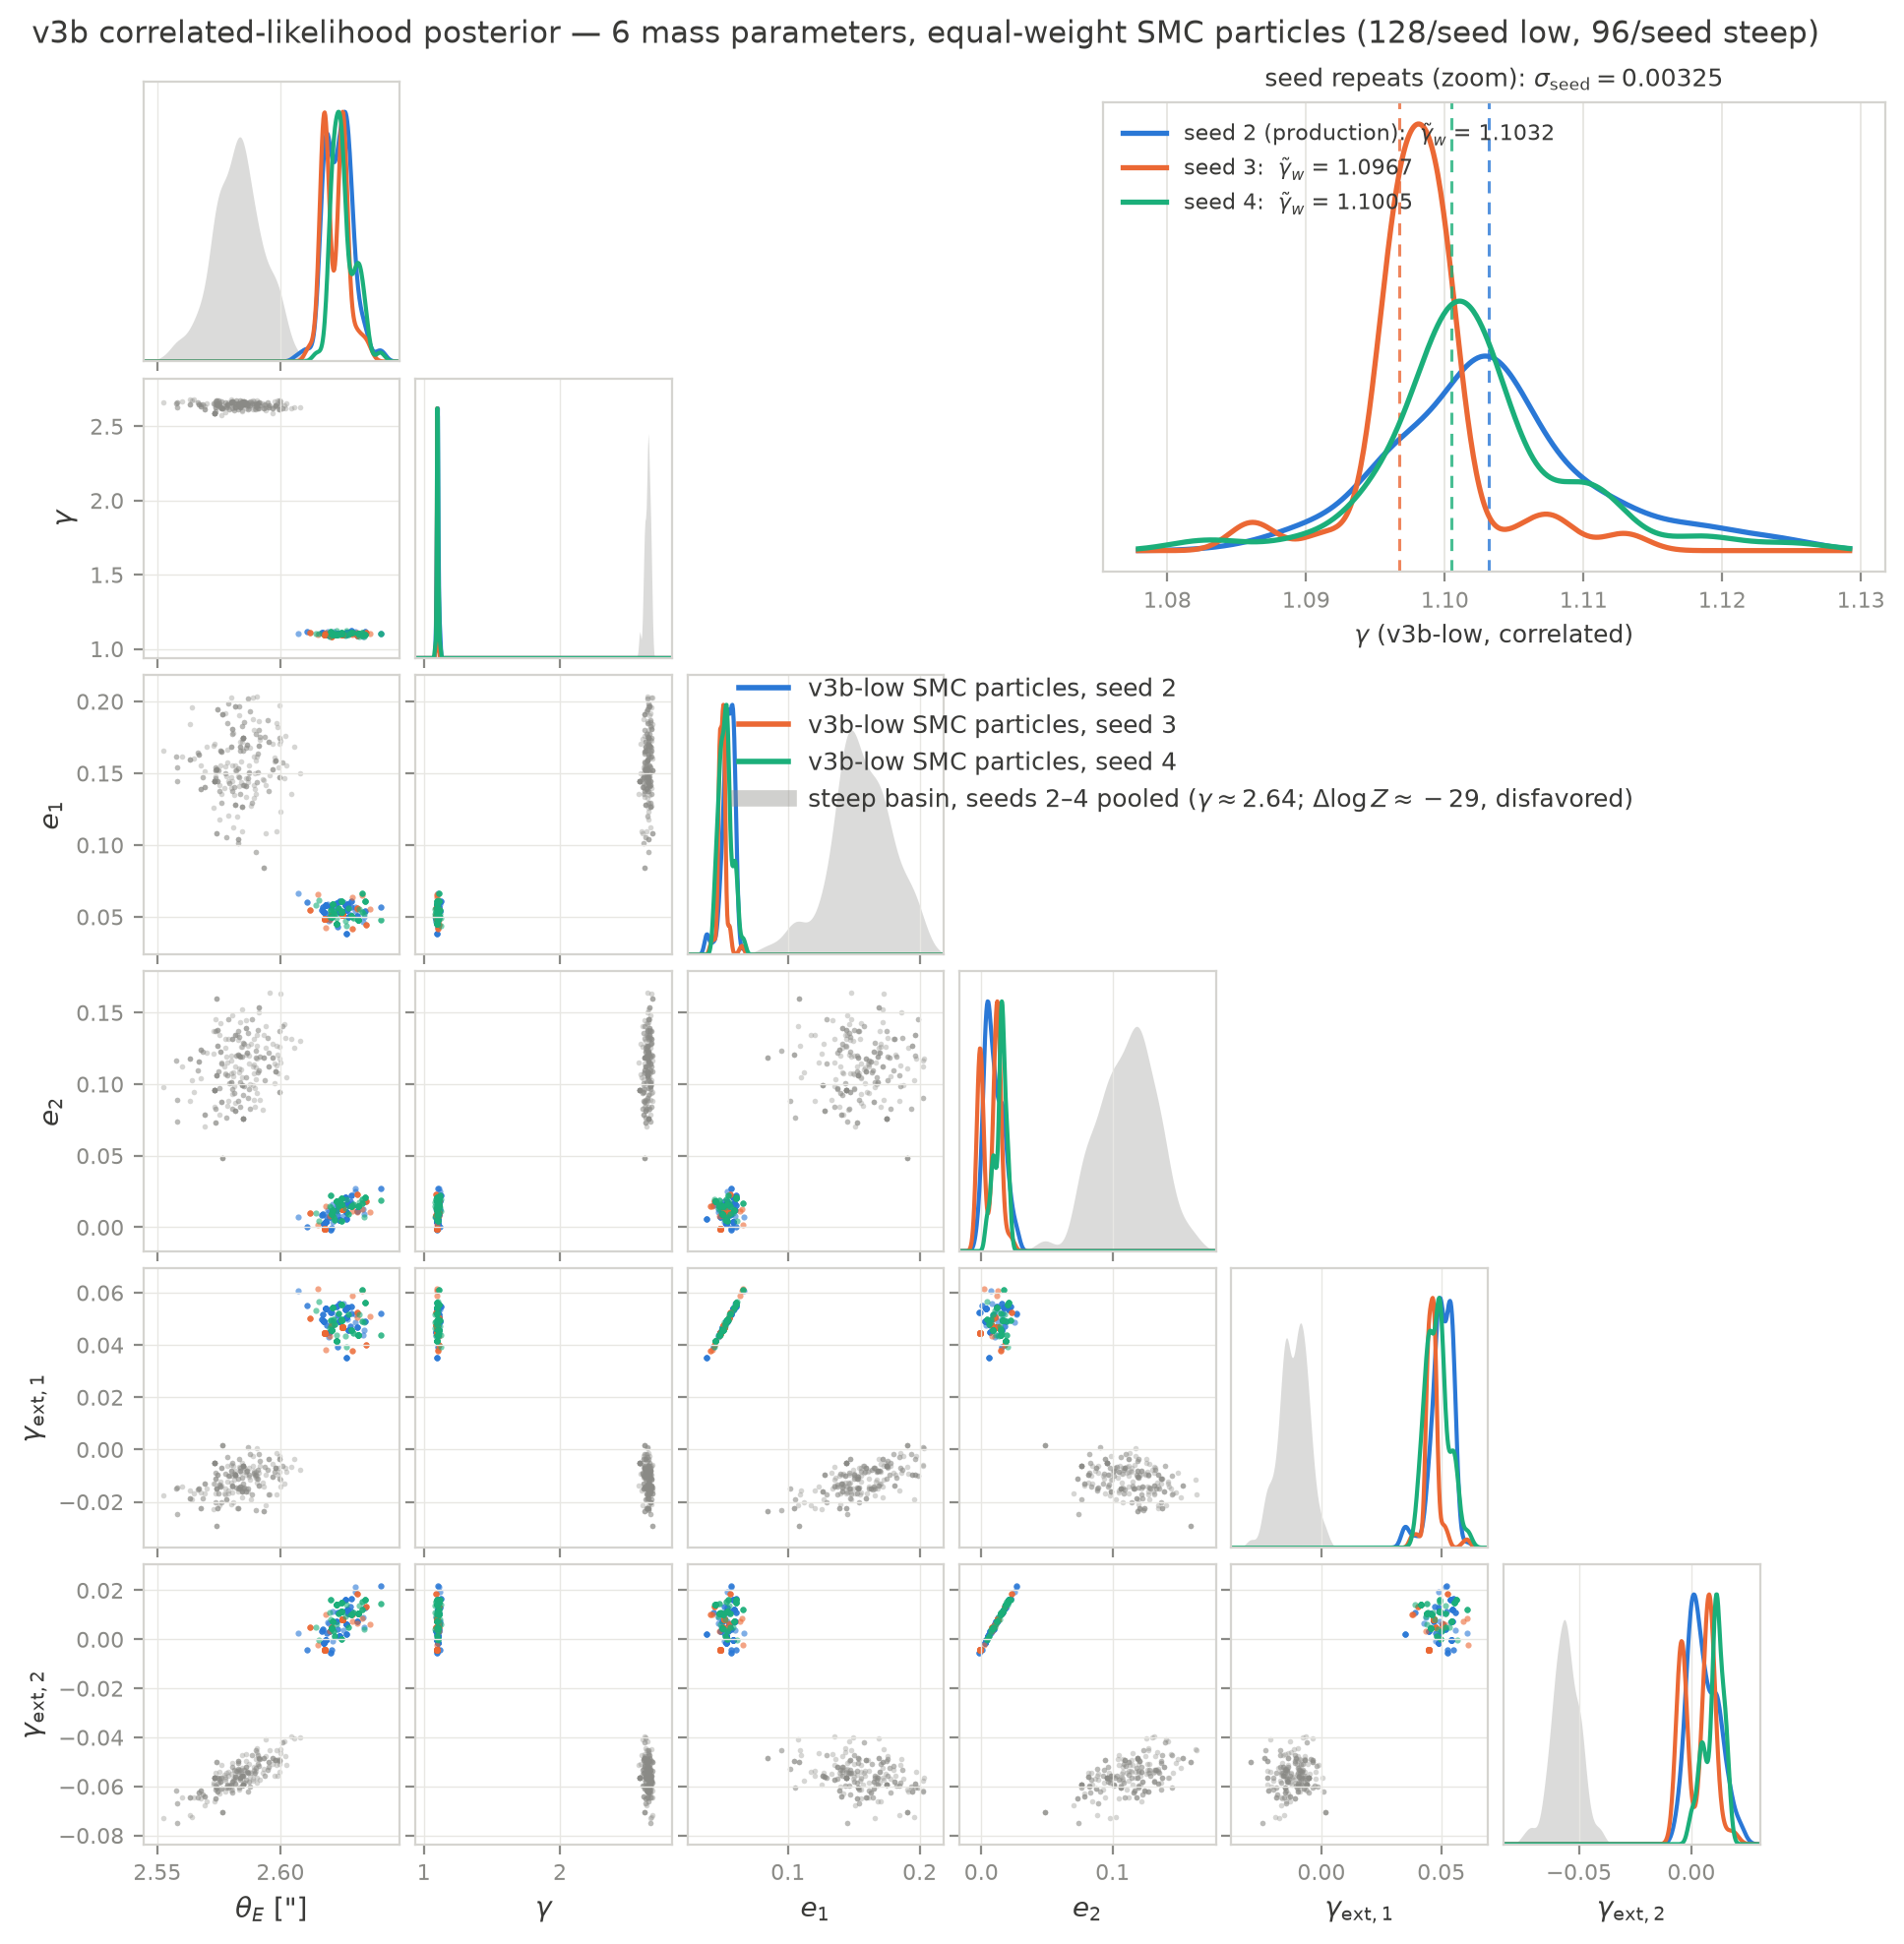
\includegraphics[width=0.98\textwidth]{../figs/rfig_corner.png}
\caption{Posterior corner of the six mass parameters (\thetaE,
$\gammaEPL$, \eone, \etwo, $\gamma_{\mathrm{ext},1}$,
$\gamma_{\mathrm{ext},2}$) from the stored equal-weight \dfile{v3b}-low
correlated SMC particles, seeds $\{2,3,4\}$ overlaid --- the SMC
convergence visual (SMC has no \Rhat; the seed-repeat spread
$\sseed=0.00325$ plus the per-stage ESS/acceptance diagnostics of
Table~\ref{tab:conv-modelers} are the analogues). Grey: the steep basin
(seeds 2--4 pooled, $\gammaEPL\approx2.64$; evidence-disfavored by
$\approx29$--$32$ nats). Inset: $\gammaEPL$ zoom with the per-seed
weighted medians of record $\{1.1032, 1.0967, 1.1005\}$; the equal-weight
particle medians reproduce them to $\le0.0027$, well inside
$\sigma_{\rm stat}=0.008$. Source artifacts: companion
\dfile{data/results/e2\_v3b\_low\_smc\_canary\_fix.json} (+ seed-3/4
repeats), \dfile{data/t02\_t03\_gate\_eval.json},
\dfile{data/rfig\_modeler\_params.npz}.}
\label{fig:corner}
\end{figure}


%%%%%%%%%%%%%%%%%%%%%%%%%%%%%%%%%%%%%%%%%%%%%%%%%%%%%%%%%%%%%%%%%%%%%%%%%%%%%%%
\section{Introduction}
\label{sec:intro-a}
%%%%%%%%%%%%%%%%%%%%%%%%%%%%%%%%%%%%%%%%%%%%%%%%%%%%%%%%%%%%%%%%%%%%%%%%%%%%%%%

\subsection{Two lineages}

The companion campaign \citep{cgl2026companion} attacked the two
ingredients that the code-comparison literature flags as under-addressed in
fast GPU lens modeling \citep{etherington2024codecomparison}: correlated
image noise and honest posterior multimodality. It delivered a validated
drizzle-anchored correlated-noise likelihood
($C=D^{1/2}KD^{1/2}$, convolutional whitening gated at operator-norm
flatness $\eop\le0.02$, generalized ridge marginalization with the Gaussian
Occam term) and the first systematic sampler benchmark on strong-lens
posteriors. On the real system \foundry\ \citep{huang2025foundry1} the
verdict was \emph{necessary but not sufficient}: the correlated likelihood
flips the binned-product bimodality --- per-basin evidence swings
$\sim$191 nats, from $\dlogZ=+162$ (diagonal) to $-29$ (correlated),
showing the upsampled steep basin to be a noise-covariance artifact --- but
over-corrects the slope, restoring a low basin at
$\gammaEPL=1.103\pm0.008$ that sits $\sim$$17\sigma$ \emph{below} the
$1.433$ native-diagonal anchor, so that the correlated slopes across pixel
scales \emph{bracket} the anchor rather than unifying onto it. Explaining
that bracket --- and certifying the machinery on which any explanation
would run --- is unfinished business this campaign inherits. On the
inference axis, the companion campaign found that the two hardest real
posteriors (a 46-dim condition-$10^{14}$ marginalized target and a 74-dim
bimodal target) defeat off-the-shelf samplers, and that per-basin tempered
SMC evidence is the only trustworthy mode-weight instrument.

Independently, the \gigalens\ team --- authors of the original GPU
recipe \citep{gu2022gigalens} and its multi-node successor
\citep{huang2026gigalens2} --- has been rebuilding the library on what we
refer to throughout as \emph{the upstream development branches}: a
JAX-only rewrite \citep{bradbury2018jax} around a unified ``\sceneapi''
(multi-plane, multi-band scene composition; a documented
\texttt{Dataset}/\texttt{LikelihoodTerm} seam; a physicality layer;
experimental microcanonical sampler kernels). Three facts about the commit
we vendored (\S\ref{sec:substrate-a}) motivate the bridge. First, its
validation suite was present but \emph{unrun} --- the forward model had no
external certification. Second, it contains no correlated-noise
likelihood, no analytic source marginalization with an Occam term, and no
tempering/SMC evidence layer --- precisely the assets the companion
campaign validated on the old stack. Third, its likelihood seam is
documented and stable enough to carry an upstream-shaped port. Per the
campaign's collision rules (\S\ref{sec:protocol-a}) we do not characterize
any unpublished results of those branches; where campaign cells ran on
data or targets provided by the team (the 33-dim multi-plane ``carousel''
cell on real MUSE cutouts), the data were \emph{provided by the team and
used with permission, with any comparison against their own runs deferred
pending their sign-off}.

\subsection{Campaign goals}

The campaign (branch \texttt{claude-giga-lens-linus}; plan frozen before
any GPU spend) set five goals:

\begin{enumerate}
\item \textbf{Certify the substrate.} Cross-stack parity of the \sceneapi\
  forward model against the validated companion-campaign stack, at
  machine precision, on both campaign machines (gate battery F1--F8,
  \S\ref{sec:substrate-a}).
\item \textbf{Port the payload.} An upstream-shaped
  \texttt{CorrelatedImageData} likelihood term on the documented
  likelihood seam, exact in its analytic limits, plus a
  mutation-kernel-generalized tempered-SMC evidence layer (MC-SMC,
  \S\ref{sec:port-a}); then the acid test: does the new substrate
  \emph{reproduce} the companion campaign's money number
  $\gammaEPL=1.103$ and its evidence at posterior level?
\item \textbf{Benchmark the bet.} A pre-registered decision matrix for
  prior-seeded MAMS-SMC against warm MAMS-alone, MCLMC, and the classic
  MAP$\to$SVI$\to$HMC recipe, across analytic, synthetic-scene,
  double-source-plane, high-condition, bimodal, and real multi-plane
  target classes --- with two-sided honest predictions written before the
  runs.
\item \textbf{Close mechanism suspects.} Why does the correlated
  likelihood over-correct? Free (0 GPU-h) and cheap discriminators for the
  profile-curvature, companion-galaxy, spectrum-flooring, and
  noise-stationarity suspects, then a confirmatory injection-recovery
  test on the real noise field.
\item \textbf{Arbitrate the anchor, and hand off.} A two-stack
  end-to-end check of the $1.433$ premise itself; and a claims-register
  handoff to the team (certification evidence, port, a first formal
  simulation-based-calibration \citep{talts2018sbc} run of the pipeline
  class, ops lessons), every scene-substrate verdict labeled
  \emph{proposed (UNCERTIFIED --- external)}.
\end{enumerate}

\subsection{Findings in brief (two-sided by design)}

House style holds honest negatives to be first-class results; we summarize
both signs here and expand in the results sections that follow.

\textbf{Certification delivered.} F1--F8 pass at machine precision on both
machines (forward image $5.7\times10^{-15}$ relative; constrained-space
gradients $1.5\times10^{-11}$), \emph{given} three documented convention
reconciliations applied on our side of the fence with the vendor
unpatched --- the largest a real $\sim$$2\times10^{-3}$ model-level
difference between the two stacks' S\'ersic $b_n$ approximants. One gate
(F6, the Occam log-determinant) required a signed, ledgered restatement
against $\mathrm{fp}128$ truth after the original cross-algorithm
reference was measured to be noisier than the tolerance it enforced
(\S\ref{sec:f6}).

\textbf{The port reproduces cross-stack.} The ported correlated term is
exact in its analytic limits (delta-kernel identity to $5.8\times10^{-11}$;
dense-Cholesky reference to $5.5\times10^{-12}$ nats) and, run end-to-end
on the new substrate on an independent machine, reproduces
$\gammaEPL_{\rm low}=1.1005$ (offset $0.0027$ against the certified
$1.1032\pm0.0086$), $\logZ$ to $0.11$ nats in the low basin and $0.37$
nats in the steep, and the low-basin
evidence preference at seed-family magnitude ($\dlogZ=-29.36$ against
$-28.9/-32.3/-31.2$). The companion campaign's headline number now stands
on two independent stacks.

\textbf{The benchmark maps capability boundaries.} Prior-seeded MAMS-SMC
is the only vehicle that produced $\logZ$ at all in this campaign, and its
failures are uniformly \emph{cost walls on a healthy sampler}, never
divergence or collapse. The classic single-stage recipe, at frozen
settings, produced zero accepted posteriors campaign-wide --- including a
faithful reproduction, on the new substrate, of the known
condition-$10^{14}$ single-stage pathology ($\Rhat_{\rm worst}=44.3$, all
chains prior-railed). The carousel-class real-data cell defeats
\emph{both} vehicles at matched budget (0 posterior draws each). MCLMC
mutations are demoted for evidence: a $20.1\sigma$ bias screen and a
$\times56$ minor-mode inflation that resampling does not launder at point
estimate. Two
cross-cutting findings bind all future evidence gates: bootstrap $\logZ$
uncertainties understate true errors (measured $+3.06\pm0.35$ nats across
an exact reparameterization where the truth is $\approx$0), and one of our
own frozen references was indicted by the very gate it anchored --- an
$11\sigma$ failure decomposing into \emph{more} evidence in both basins
with $\gammaEPL$-disjoint ensemble support, i.e.\ a within-basin coverage
defect in the reference, not (only) the vehicle.

\textbf{Stationarity rejected; mechanism standing but unconfirmed.} The
stationary noise-kernel class behind $\gammaEPL=1.103$ is provably
violated by the real field (calibrated $p=0.010$, replicated with the arc
excluded; cross-block kernel spread $16.4\times$ the drizzle-registration
envelope), while the cheap alternatives died: profile curvature is
structurally dead at zero GPU cost, the companion galaxy is exonerated
($-0.0021$ shift), and spectrum flooring is rejected by thousands of nats.
The confirmatory injection-recovery test returned NO-CONFIRM /
NO-EXONERATE: positive-signed biases outside both pre-registered zones
with a control that failed high \emph{and} sick, implicating the injection
construction (scene-subtraction residue) under the pre-registered honesty
clause. Noise-model-class misspecification remains the working
hypothesis --- unconfirmed, unrefuted.

\textbf{Arbitration bounded, not decided.} The two-stack anchor check
exhausted four vehicles without producing a quotable $\gammaEPL$ on the
46-dim diagonal target; it closed PARTIAL-BY-VEHICLE-EXHAUSTION, with the
premise carried indirectly by machine-precision likelihood parity (F1--F6)
plus the \emph{converged} correlated-target reproduction above. ``$1.433$
reproduces at posterior level on the new substrate'' is therefore
\emph{untested}, and is flagged as such wherever the anchor is used.

The remainder of this report: \S\ref{sec:substrate-a} (substrate and
certification battery), \S\ref{sec:port-a} (correlated likelihood port and
the MC-SMC evidence layer), \S\ref{sec:protocol-a} (protocol, labeling,
and budget fences), followed by the results sections (benchmark decision
matrix; mechanism program; cross-stack reproduction and arbitration;
gifts and handoff), the discussion of open items, and the reproducibility
appendix.

%%%%%%%%%%%%%%%%%%%%%%%%%%%%%%%%%%%%%%%%%%%%%%%%%%%%%%%%%%%%%%%%%%%%%%%%%%%%%%%
\section{Methods I: Substrate, Environment, and Cross-Stack Certification}
\label{sec:substrate-a}
%%%%%%%%%%%%%%%%%%%%%%%%%%%%%%%%%%%%%%%%%%%%%%%%%%%%%%%%%%%%%%%%%%%%%%%%%%%%%%%

\subsection{Vendored substrate and pinned environment}

The campaign runs against a frozen snapshot of the upstream development
branch, vendored at commit \vendorpin\ (full SHA in
\dfile{vendor/gigalens-linus/VENDORED\_REF.txt}) via \texttt{git archive}
--- \emph{unpatched}, installed \texttt{--no-deps}. Every campaign process
asserts the vendor identity at import (\texttt{require\_vendor\_ref}), and
a ledgered re-pin procedure (motivation $\to$ re-archive $\to$ diff review
of the three subclassed surfaces $\to$ full gate-battery re-run green)
guards against silent drift of the moving branch; it was never needed ---
the pin held for the whole campaign. All campaign-side adaptation lives in
the shim package \dfile{cgl2/} (parameter mapping, guards, scene factories,
the correlated term, and the samplers); the vendor tree was never edited.

Table~\ref{tab:pins-a} lists the pinned environment. The single deviation
from the upstream declared pins --- numpy 2.4.6 versus their 2.1.3 --- is
recorded as a known deviation and covered by the gate battery. The old
validated stack \citep[commit \texttt{58ec9a7};][]{cgl2026companion} is
imported by path, never copied; whitener bundles and Foundry-I data
products likewise. Production GPU cells ran single-GPU shared-QOS on NERSC
Perlmutter A100s; certification and free checks ran on the local phoenix
node (L4/A16).

\begin{table}[htbp]
\centering\small
\caption{Pinned software environment (venv \texttt{cgl2}, mirrored as
\texttt{cgl2-pm} on Perlmutter). Pins are seeded from the companion
campaign's \texttt{constraints.txt}; all installs are constrained.}
\label{tab:pins-a}
\begin{tabular}{lll}
\toprule
Component & Version & Note \\
\midrule
python & 3.13 & \\
jax / jaxlib & 0.6.2 & upstream's declared pin; identical on both machines \\
\blackjax & 1.3 & \citep{blackjax2024} \\
tensorflow-probability & 0.25.0 & \citep{dillon2017tfp} \\
numpy & 2.4.6 & \emph{known deviation} vs.\ upstream 2.1.3; gate-covered \\
tensorflow & --- & absent; the vendored dependency is verified inert \\
vendor & \vendorpin & UNPATCHED; \texttt{--no-deps}; identity-guarded \\
old stack & \texttt{58ec9a7} & validated companion-campaign stack, by path \\
\bottomrule
\end{tabular}
\end{table}

\subsection{Reference-artifact parity design}

Both stacks ship as a Python package named \texttt{gigalens}, so the
originally planned single-process dual import is impossible (a name
collision the upstream documentation itself warns about). The enacted
design (ledgered decision D3) is \emph{reference-artifact parity}: the old
validated stack, running in its own certified virtual environment, dumps
reference arrays (forward images, design-matrix columns, log-likelihoods,
constrained-space gradients) to \dfile{data/parity\_refs.npz} for the
foundry v2d and v3b inputs at a reference point $z_{\rm ref}$ plus three
seeded perturbations; the \sceneapi\ stack then recomputes the identical
quantities in the campaign environment and compares. Both sides run the
same jax 0.6.2, which preserves $10^{-12}$-class comparability across the
process boundary. Comparison is \emph{in constrained parameter space}
through the campaign's name-keyed parameter map (never positional
ordering), so any flat-vector convention bug fails parity by construction.

\subsection{The F1--F8 certification battery}

Table~\ref{tab:gates-a} gives the battery and its frozen thresholds
(fixed at P0, before any science ran); the measured results, on both
machines, are reported with the certification results in \S\ref{sec:cert}
(Table~\ref{tab:parity}). F1--F4 constitute, to our knowledge, the first
external certification evidence for the \sceneapi\ forward model in the
EPL+shear + 4$\times$S\'ersic / S\'ersic+shapelets ($n_{\max}=6$)
configuration class --- the vendored validation suite was unrun at the
pin. F8 repeats the entire battery under the Perlmutter-native pinned
environment on an A100, so that the stack is certified on both machines
before any production cell. Parity at these thresholds holds \emph{given}
three documented convention reconciliations, applied on our side of the
seam with the vendor unpatched; they are themselves findings and are
reported with the results (\S\ref{sec:conventions}).

\begin{table}[htbp]
\centering\footnotesize
\setlength{\tabcolsep}{4pt}
\caption{Cross-stack certification battery design: old validated stack
(\texttt{58ec9a7}) versus the \sceneapi\ (\vendorpin), same foundry
\dfile{v2d}/\dfile{v3b} inputs, $z_{\rm ref}$ + 3 seeded perturbations,
constrained-space comparison, scored on the worst case over products and
perturbations. Thresholds frozen at P0; F6 is quoted under its restated
form (\S\ref{sec:f6}). Measured results: Table~\ref{tab:parity} and
\S\ref{sec:cert}--\S\ref{sec:corrport}.}
\label{tab:gates-a}
\begin{tabular}{@{}lll@{}}
\toprule
Gate & Statement & Threshold \\
\midrule
F1 & forward image & $\le10^{-12}$ rel \\
F2 & design-matrix columns & $\le10^{-12}$ rel \\
F3 & diagonal masked loglik + $\chi^2$ & $\le10^{-8}$ \\
F4 & grad of marg.\ loglik (constrained) & $\le10^{-8}$ rel-$L_2$ \\
F5 & delta-kernel corr.\ term $\equiv$ stock & $\le10^{-10}$ \\
F6 & Occam $-\tfrac12\log\det A$ vs fp128 truth & cond-scaled (\S\ref{sec:f6}) \\
F7 & flat-$z$ round-trip + name audit & exact (info) \\
F8 & full battery, Perlmutter-native env & report-only \\
03-A & corr.\ term vs dense-Cholesky ($32^2$ toy) & $\le0.1$ nat \\
03-B & delta identities (fwd; conv$\equiv$multiply) & $\le10^{-10}$ \\
W & whitener-bundle revalidation & $\eop\le0.02$ strict \\
\bottomrule
\end{tabular}
\end{table}

The whitener bundles imported from the companion campaign were revalidated
in place (gate W): operator-norm flatness $\eop$ reproduced exactly,
erosion masks reproduced from first principles, kernel hashes pinned. The
three production bundles (v2d, v3b, v3) are admissible under the strict
$\eop\le0.02$ gate; the ledgered relaxed arm \texttt{v2d\_relaxed}
($\eop=0.0312$ against its own design target $0.05$) is correctly
\emph{inadmissible-by-design} and fenced from production
use.\art{data/whitener\_manifest.json}

%%%%%%%%%%%%%%%%%%%%%%%%%%%%%%%%%%%%%%%%%%%%%%%%%%%%%%%%%%%%%%%%%%%%%%%%%%%%%%%
\section{Methods II: The Correlated-Noise Likelihood Term and the MC-SMC
Evidence Layer}
\label{sec:port-a}
%%%%%%%%%%%%%%%%%%%%%%%%%%%%%%%%%%%%%%%%%%%%%%%%%%%%%%%%%%%%%%%%%%%%%%%%%%%%%%%

\subsection{\texttt{CorrelatedImageData}: an upstream-shaped port}
\label{sec:corr-port-a}

The correlated-noise payload is ported as a dataset class
\texttt{CorrelatedImageData} with its companion likelihood term
\texttt{Correlated\allowbreak Image\allowbreak Likelihood\allowbreak Term}
(\dfile{cgl2/correlated.py}), subclassing the \sceneapi's documented
\texttt{Dataset} and \texttt{LikelihoodTerm} seam --- shaped so that
upstream adoption is a move, not a rewrite. Design points, each carrying a
validation gate:

\begin{itemize}
\item \textbf{Frozen whitener bundles as data.} The constructor takes a
  frozen whitener bundle (convolution taps, $D^{-1/2}$ diagonal, eroded
  keep-mask, $\eop$, kernel hash) and validates it
  raise-never-default; \texttt{event\_size} is the kept whitened degrees
  of freedom. The whitener seam is deliberately pluggable: the
  stationarity rejection (\S\ref{sec:intro-a}) means a locally-stationary
  (per-region) kernel class is the anticipated successor, and the term is
  agnostic to which bundle it is handed.
\item \textbf{Single-render contract.} One basis render per likelihood
  evaluation, via \texttt{lstsq\_simulate} with
  \texttt{return\_stacked=True}, honoring the upstream single-forward-eval
  contract and reusing the fused convolution/pooling path verbatim;
  residual and design columns are whitened by a grouped depthwise
  convolution wrapped in \texttt{jax.checkpoint} (the memory fix that
  keeps SMC particles under the $\le$200\,MB budget). Masked operations
  use \texttt{jnp.where}, never multiplication by a mask.
\item \textbf{Ridge marginalization with the Occam term.} The linear
  (shapelet) amplitudes are analytically marginalized under a generalized
  ridge prior, \emph{including} the $-\tfrac12\log\det A$
  Gaussian-evidence term that a plain linear solve omits --- the term that
  makes downstream Bayes factors meaningful. Whitened $\chi^2$ is exposed
  through the upstream \texttt{reports\_chi2} channel.
\item \textbf{Exactness in analytic limits.} With a delta kernel the
  term reduces exactly to the stock
  \texttt{Image\allowbreak Likelihood\allowbreak Term} (F5:
  $5.8\times10^{-11}$; conv$\equiv$multiply identity $0.0$); on a $32^2$
  toy with a dense covariance it matches an exact Cholesky reference to
  $5.5\times10^{-12}$ nats against a 0.1-nat gate
  (03-A).\art{data/correlated\_term\_validation.json} Production wiring
  adds an old-vs-new whitened marginalized log-likelihood/gradient
  cross-stack check at $z_{\rm ref}$ plus three seeded perturbations
  (worst $|\Delta\log L_{\rm marg}|$: $2.4\times10^{-8}$ on \dfile{v2d},
  $7.2\times10^{-7}$ on
  \dfile{v3b})\art{data/parity\_report\_scene.json} and a
  remat-exactness gate (checkpointed vs.\ un-checkpointed whitening,
  difference exactly $0.0$).\art{data/l0\_remat\_gate.json} Separately,
  B0's target-adapter parity gate compares old and new log-densities at
  64 prior draws (max $|\Delta|$ exactly
  $0.0$).\art{data/smc\_b0\_report.json}
\end{itemize}

For SMC the likelihood is evaluated in f64: a f32 forward path carries a
$\sim$0.3-nat evaluation noise floor that would pollute
Metropolis--Hastings acceptance in the mutation kernels.

\subsection{MC-SMC: tempered SMC with microcanonical mutation kernels}
\label{sec:mcsmc-a}

The evidence layer (\dfile{cgl2/samplers/smc\_micro.py}) generalizes the
companion campaign's validated adaptive tempered-SMC driver
\citep{delmoral2006smc} --- the \sceneapi's \texttt{ProbModel} log-prior
/ log-likelihood split maps exactly onto the \blackjax\ convention ---
with the mutation kernel abstracted over three choices:

\begin{itemize}
\item \textbf{HMC} --- the proven baseline from the companion campaign.
\item \textbf{MAMS} \citep{robnik2024mams} --- the \emph{primary} and the
  campaign's bet: Metropolis-adjusted microcanonical dynamics, whose
  exact $\pi_\lambda$-invariance at every tempering stage is what makes
  the SMC evidence estimate unbiased.
\item \textbf{MCLMC} \citep{robnik2023mclmc} --- unadjusted microcanonical
  dynamics, admitted \emph{diagnostic-only} behind a pre-registered bias
  gate (below), never as an evidence kernel.
\end{itemize}

Kernel logic is copied with attribution from the upstream experimental
implementations, never imported (those modules reach into private
\blackjax\ internals and the pre-rewrite simulator). Per-$\lambda$ tuning
was frozen at P0, before any science cell: mass matrix from the
regularized weighted particle covariance; step size from a short
dual-averaging pilot per stage (10 iterations, acceptance target 0.90 for
MAMS per the MAMS integrator recommendation, 0.80 for HMC; an
energy-variance-per-dimension pilot for MCLMC); 4 kernel draws per stage;
adaptive $\lambda$-schedule by bisection on the incremental-weight ESS at
target $0.7N$ with systematic resampling; $\logZ$ accumulated per stage
with a per-stage bootstrap error \sboot. Gradient evaluations are
ledgered exactly (pilot draws billed identically), which is what makes the
budget-matched benchmark arms of the results sections well-defined.

\textbf{B0 correctness gates (frozen at P0).} On analytic targets the
layer passes where it must and fails where the class fails, and both are
recorded:\art{data/smc\_b0\_report.json} target adapters build 11/11; on
the 2-dim bimodal \texttt{mix2}, $|\logZ$ error$|=0.073\le3\sboot$ with
minor-mode weight $0.219$ against truth $0.2$; on the 46-dim
ill-conditioned target the worst-parameter $|z|=1.83$ passes while the
$\logZ$ error is $2.40$ nats at $\sboot=0.37$ --- i.e.\ $6.6\sigma_{\rm
boot}$, the first measurement of the campaign-wide finding that
\emph{bootstrap $\logZ$ errors understate true errors on ill-conditioned
targets}; on \texttt{funnel10} the layer \emph{fails} ($-0.66$-nat $\logZ$
deficit) --- a pre-existing limitation of the adaptive tempered-SMC class,
reproduced in the old validated stack and carried as a caveat, not a port
defect. The pre-registered MCLMC bias screen fired: MCLMC-vs-MAMS
$\dlogZ=+10.79\pm0.54$ on the ill-conditioned target, i.e.\
$20.1\sigma$,\footnote{The ledger prose records ``$30\sigma$''; the
artifact of record \dfile{data/smc\_b0\_report.json} gives
$10.79/0.536=20.1$. Per the campaign's discrepancy-flag rule
(\S\ref{sec:protocol-a}) the artifact value is quoted; the demotion
($>3\sigma$ rule) is unaffected.} demoting MCLMC to
diagnostic/cost-frontier-only for the entire campaign --- a demotion whose
independent confirmation ($\times56$ minor-mode evidence inflation on the
74-dim bimodal target) appears in the results.

\subsection{The checkpoint/resume retrofit}
\label{sec:ckpt-a}

The benchmark's first production wave lost $\sim$17.6 of its 18.7
A100\,h to zero-artifact timeouts (only 1.12\,h produced readable
science): the frozen SMC driver wrote results only at
$\lambda=1$ and printed no stage progress, so wall-capped jobs burned
silently. The response --- kept out of the frozen driver, which was never
edited --- is a checkpointing retrofit
(\dfile{cgl2/samplers/ckpt.py}) with three properties:

\begin{enumerate}
\item \textbf{Per-stage full state.} A delegating
  \texttt{CheckpointKernel} (build/tune/mutate verbatim) writes a
  full-state checkpoint per $\lambda$-stage (post-mutation particles,
  $\lambda$, step size, trajectory length, acceptance, and the exact
  per-stage gradient/log-probability ledger) plus one progress line; a
  pre-registered in-job wall cap raises \emph{after} the checkpoint, with
  an exit-3 PARTIAL protocol --- a wall hit preserves progress by
  construction, and no gate math is ever run on a non-$\lambda{=}1$
  ensemble.
\item \textbf{Evidence-complete resume.} Weight-stage log-likelihoods are
  recorded through the driver's existing \texttt{loglik\_batch\_fn} seam
  (delegation only), so a resumed run retains the \emph{full} $\logZ$
  accumulation and per-stage bootstrap --- not a partial-from-resume
  approximation.
\item \textbf{Bit-identity.} On \texttt{--resume}, the RNG chain is
  fast-forwarded by replay of the recorded log-likelihoods; the retrofit
  gate proves a fresh run and an interrupted-then-resumed run
  \emph{bit-identical} including $\logZ$ and its bootstrap, and that
  resume-after-completion rebuilds the identical result with zero new
  forward evaluations. (Documented caveat: under strict-f32 execution the
  checkpointed ensemble is an f64 reconstruction of the f32 state, so
  resume there is protocol-identical up to an f32-rounding-level
  perturbation; everywhere else it is bit-exact.)
\end{enumerate}

The retrofit ships with a 58-test suite, green on both machines. Its
operational effect is visible throughout the results: the recovery lane
turned the first wave's zero-artifact failure mode into readable
recoveries (3 of 4 cells), and the 12-hour, three-leg chained real-data
carousel run --- and every partial-$\lambda$ cost readout quoted in the
decision matrix --- exists only because interrupted evidence runs became
resumable and readable at all.

%%%%%%%%%%%%%%%%%%%%%%%%%%%%%%%%%%%%%%%%%%%%%%%%%%%%%%%%%%%%%%%%%%%%%%%%%%%%%%%
\section{Methods III: Protocol}
\label{sec:protocol-a}
%%%%%%%%%%%%%%%%%%%%%%%%%%%%%%%%%%%%%%%%%%%%%%%%%%%%%%%%%%%%%%%%%%%%%%%%%%%%%%%

\subsection{Pre-registration and frozen gates}

Every experimental cell was preceded by a \emph{design checkpoint} logged
to the campaign record before submission: hypothesis, predicted direction
and magnitude, falsifier, and derived threshold. Certification gates
(F1--F8, B0) were frozen at P0 in the repository README before any
science ran. Thresholds parameterized by then-unknown quantities carried
declared placeholders that were \emph{finalized, not moved}, when the
parameterizing measurement landed: the seed-repeatability study fixed
$\sseed(\gammaEPL)=0.00325$ (low basin), $0.00664$ (steep), and
$\sseed(\dlogZ)=1.79$ nats (with the $n{=}3$ caveat --- $\pm46\%$
$\chi$-distribution sampling error --- quoted at every use), and the
downstream gates inherited these by a ledgered finalization
row.\art{data/t02\_t03\_gate\_eval.json} Where a pre-registered gate
proved undecidable as written, the record shows the branch taken rather
than a rescored verdict: outcomes in this report include
FAIL-as-written, NOT-DECIDABLE-AS-REGISTERED, PARTIAL-BY-BUDGET,
NOT-EVALUABLE-WITHIN-BUDGET, and AMBIGUOUS-AT-FROZEN-THRESHOLDS ---
honest negatives are first-class results, and no threshold was moved
after data. Two further house rules: diagnostic figures are produced and
inspected \emph{before} gate text is written (a rule adopted from the
upstream team's research culture), and amendments (a re-registered gate,
a descoped cell) enter the record as explicit ledgered decisions with the
original always preserved.

\subsection{Proposer $\ne$ grader: the UNCERTIFIED-external label}

The campaign separates producing a result from certifying it. For every
claim that runs through the \sceneapi\ substrate, we are the
\emph{proposer}; the \emph{grader} is the upstream \gigalens\ team (and
Greg Benson for our-side scope). Accordingly, every scene-substrate
verdict in this report carries the label \emph{proposed (UNCERTIFIED ---
external)}, and the deliverable of record is a claims register in the
team's own lab-notebook format
(\dfile{papers/handoff/CLAIMS.md}: fourteen claims, each with
pre-registered criterion, measured numbers, named artifacts, and a
mandatory doubt report). ``Validated'' is reserved, throughout this
report, for the old certified stack; scene-API results are
``reproduced/measured, UNCERTIFIED (external).'' Claims derived from data
or targets provided by the team are additionally marked SIGN-OFF GATED in
the register: internal-memo material, publication-gated on the team's
explicit sign-off. In this report the carousel real-data cell appears
under exactly that regime --- \emph{data provided by the team, used with
permission; any comparison against their own runs is deferred pending
sign-off} --- and the upstream repositories are referenced only as the
upstream development branches, without characterization of their
unpublished results.

Four bright lines, frozen in the plan before the campaign began, bind the
published text: (i) no result is presented so as to be readable as an
MCLMC-vs-HMC efficiency comparison on a unimodal target --- every sampler
number in this report attaches to a multimodality, evidence, cold-start,
or noise-model question; (ii) nothing derived from the upstream branches'
unpublished code or results appears externally without the team's
sign-off; (iii) the team's ongoing staged campaigns are untouched --- our
prototypes are offers, not applications; (iv) co-authorship is offered on
any publication whose results run through their substrate.

\subsection{Budget fences and operational discipline}

The campaign ran under a 100 A100\,h hard stop with per-phase caps and a
ledger-before-results rule: the estimated cost of every job is appended to
the campaign ledger \emph{before} any result is read, and actuals are
harvested from \texttt{sacct}. Realized spend was 53.51 A100\,h ---
certification slice 2.21, injection-recovery 7.80, benchmark 22.45 of a
24-h cap, the user-funded real-data extension 15.85 of 18, and the
payload/arbitration phase 5.21 of 17 (component sums differ from the
total by 0.01\,h of per-row rounding).\art{CAMPAIGN.md (A100-hour
ledger)} Sub-fences were binding, not advisory: chained runs carried
per-leg wall caps with pre-declared stop conditions (the carousel chain
stopped at its fence with $\lambda=0.15$, and the cell was closed by an
explicit ledgered decision, D9, rather than extended), budget-matched
comparison arms were
capped at their partner's \emph{realized} gradient ledger, and cells
whose measured cost exceeded remaining headroom closed as
NOT-EVALUABLE-WITHIN-BUDGET rather than overrun. Unused programmed items
are closed explicitly in a final gate-ledger sweep (six programmed items
proposed NOT-RUN with reasons --- among them the S7
flow-preconditioned-MAMS arm, whose prerequisite B1 $\lambda{=}1$
ensemble never came to exist, and the X3 evidence-scored Vela-ladder
prototype, never mobilized --- plus B4 proposed
NOT-EVALUABLE-WITHIN-BUDGET) rather than silently
dropped.\art{research/gate\_ledger\_final.md}

Operational rules that each cost real budget to learn once, then became
protocol: production SMC jobs pin high-memory GPUs (\texttt{-C
gpu\&hbm80g}; memory sizings measured under rematerialization do not
transfer to un-rematerialized runs); the submitted batch-script snapshot
is verified by checksum via \texttt{scontrol write batch\_script} (SLURM
snapshots the script at submission --- a ``resubmitted fix'' can silently
run the old code); every campaign file is checksum-audited on the remote
before production (single-writer manifest, union-merge on conflict); a
dead-man watchdog with per-job expected artifacts and stall alerts armed
every wave; and the lensing likelihood is never evaluated on CPU. A full
ops-lessons table, with the job ids that motivated each rule, accompanies
the reproducibility appendix.

\subsection{Provenance rule}

Every headline number in this report is traced to an on-disk artifact
(JSON/NPZ path), and where it was produced on Perlmutter, to a SLURM job
id; the campaign ledger \texttt{CAMPAIGN.md} records the gate row and the
decision context. Where the ledger prose and the artifact of record
disagree, the synthesis that feeds this report flags the discrepancy
rather than smoothing it --- seven such flags are on record, and in every
case this report quotes the \emph{artifact}
value.\art{research/synthesis\_tables.md (\S4, discrepancy flags)} The
experimental record --- plan, ledger, design checkpoints, gate
evaluations, and the claims register --- ships with the repository.

% --- end of section file A (front matter + methods I/II/III) ---
